\section{Study case: experiments and evaluation} \label{section:study-case}
%To evaluate our system we need some initial data to define the \textit{relevances} and some (real or simulated) users to test with.

To evaluate our system,  we developed a prototype\footnote{https://github.com/gustavoaca1997/datatourisme-recommender}, with Java, 
Fuseki server as the triplestore, Apache Jena for traversing the ontology and connecting to the triplestore, and a MySQL database for storing additional information of the nodes and items. To have initial data, we requested real users through questionnaires, whose information was used to  create simulated users and scenarios to test with.

With this version of RECESO, we are particularly testing the User Interest Model Module, the Recommendation Module, and the Activation Propagation algorithm from the Context Module, while the Data Gathering Module and the context gathering (Location and Context Factors) are simulated.

%The prototype system was built with Java. We used a Fuseki server as the triplestore, Apache Jena for traversing the ontology and connecting to the triplestore and a MySQL database for storing additional information of the nodes and items.

\subsection{Ontology Classes}
We consider a light version o DATATourisme ontology\footnote{http://info.datatourisme.gouv.fr/ontology/core/2.0/}, consisting of the \textit{Point of interest} class, its \textit{Place} subclass, from which we take: \textit{Cultural Site, Food Establishment, Leisure Place, Natural Heritage, Sports,} and \textit{Store}.  We slightly modified the ontology DATATourisme to specialize the class \textit{Sports and Leisure Place} into \textit{Sports} class and \textit{Leisure Place} class, hence making less ambiguous what kind of places should belong to each category. Figure \ref{fig:ontology} shows the subset of classes of DATATourisme ontology, considered  in the experiments.


\begin{figure}[h]
\centering
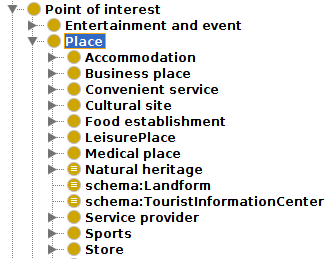
\includegraphics[scale=0.5]{ontology.png}
\caption{Subset of the modified version of the ontology DATATourisme
%(http://info.datatourisme.gouv.fr/ontology/core/2.0/)
}
\label{fig:ontology}
\end{figure}

The high level classes that are directly linked to the context factors are:
\begin{itemize}
    \item \textit{Museum}
    \item \textit{Interpretation Center}
    \item \textit{Library}
    \item \textit{Park and Garden}
    \item \textit{Archaeological Site}
    \item \textit{Religious Site}
    \item \textit{Remarkable Building}
    \item \textit{City Heritage}
    \item \textit{Defense Site}
    \item \textit{Remembrance Site}
    \item \textit{Technical Heritage}
    \item \textit{Food Establishment}
    \item \textit{Natural Heritage}
    \item \textit{Sports}
    \item \textit{Leisure Place}
    \item \textit{Store}
\end{itemize}

%\subsection{Relevances}
\subsection{From real users to simulated scenarios}
\label{section:relevances-survey}

In order to test several scenarios with different user's preferences, profiles, and behaviors,  we created synthetic scenarios, however based on data gathered from real people.
We asked people to fill a google form with two parts: 

\begin{enumerate}
    \item To determine the relevances for each context factor. The list of asked context factors included weather (with possible values {\tt rainy, cloudless, snowy}), time (with possible values {\tt early morning, morning, afternoon, night}), and day (with possible values {\tt weekday, weekend}). The list of asked types of POIs was the high level classes listed in the previous section. The question was "how much the context factor $c$ with value $v$ influences your decision to go to a 'place/event' of the type $t$ (these types are not exclusive)". People should answer an integer value between $0$ and $2$, where: 
\begin{itemize}
    \item $0$ means that if the context factor is met, you would not go to the place/event.
    \item 1 means you do not care if the context is met or not.
    \item 2 means that if the context is met, you would go to the place/event.
\end{itemize}

Then, for each pair of ontology class and context factor value (for example \textit{Museum} with \textit{rainy}), the average relevance is computed and stored as the relevance for the experiments.


 \item To determine users' preferences to tourism categories (i.e., classes of the POI ontology). In this part of the questionnaires, people provided their preferences  of high level ontology classes mentioned before, and also the genre, country, profession, age, and (optional) social networks to have more information for further work.
 
\end{enumerate}
    
    %Both for relevance and preferences, 
    We got around 100 answers from people of different ages, professions, and countries.  With this information a set of synthetic tourists is generated, with different behaviors for different context scenarios.
    


\subsubsection{Simulated scenarios}
To evaluate the system, it was decided to test it with simulated scenarios (simulated contexts and simulated users). A set of centroids of a set of clusters were chosen as the set of simulated users from the user preferences gathered before. The \textit{K-Means} algorithm was used to get the clusters and \textcolor{red}{the \textit{Elbow Method} was used to generate four clusters , since increasing this number does not make improvements worth the cost using our small dataset (see Figure \ref{fig:elbow}). In future work, a larger dataset should be used.}

\textcolor{green}{YO CREO QUE QUEDA MEJOR ASÍ: the \textit{Elbow Method} (see Figure \ref{fig:elbow}) was used to choose $4$ as the number of clusters, since increasing this number does not make improvements worth the cost using our small dataset. In future work, a larger dataset should be used.}

\begin{figure}[h]
    \centering
    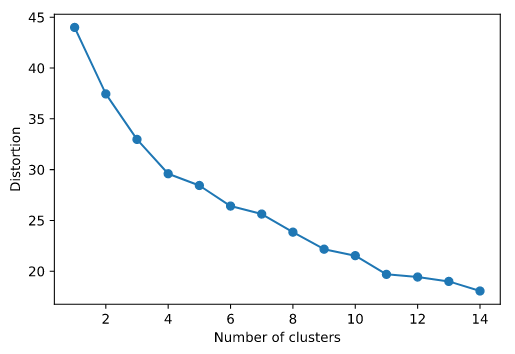
\includegraphics[scale=0.45]{elbow.png}
    \caption{Distortions of the different number of clusters}
    \label{fig:elbow}
\end{figure}

The centroids of the four clusters represent our four synthetic tourists, $T_1, T_2, T_3, T_4$. Table \ref{table:centroids} shows the preferences for each tourist to each tourism category, according our light version of DATATourise ontology.  Figure \ref{fig:tourist_hist} shows for each tourist how the preferences are distributed, where we can see that $T_3$ is the one with a more varied set of preferences, including the lowest values between all preferences.

\begin{table}[h!]
\centering
\caption{Simulated tourists' preferences}
%\caption{Centroids to be used as simulated users}
\label{table:centroids}
\begin{tabular}{ |c|c|c|c|c| } 
    \hline
    Class & $T_1$ & $T_2$ & $T_3$ & $T_4$ \\
    \hline
    \hline

    Museum & 0.7235 & 0.6476 & 0.78 & 0.9421 \\ 
    \hline
    Interpretation Center & 0.6824 & 0.6476 & 0.52 & 0.8737 \\
    \hline
    Library & 0.5588 & 0.46667 & 0.72 & 0.7684 \\
    \hline
    Park and Garden & 0.865 & 0.8714 & 0.7 & 0.9316 \\
    \hline
    Archaeological Site & 0.6882 & 0.8619 & 0.82 & 0.826 \\
    \hline
    Religious Site & 0.45882 & 0.7 & 0.36 & 0.7316 \\
    \hline
    Remarkable Building & 0.6529 & 0.8524 & 0.4 & 0.7895 \\
    \hline
    City Heritage & 0.7412 & 0.919 & 0.58 & 0.8632 \\
    \hline
    Defence Site & 0.5412 & 0.8529 & 0.68 & 0.7421 \\
    \hline
    Remembrance Site & 0.4941 & 0.781 & 0.8 & 0.7211 \\
    \hline
    Technical Heritage & 0.4059 & 0.7905 & 0.56 & 0.5842 \\
    \hline
    Food Establishment & 0.9059 & 0.8905 & 0.7 & 0.6632 \\
    \hline
    Natural Heritage & 0.9059 & 0.9143 & 0.76 & 0.9211 \\
    \hline
    Sports & 0.9353 & 0.8429 & 0.22 & 0.6316 \\
    \hline
    Leisure Place & 0.9353 & 0.8429 & 0.22 & 0.6316 \\
    \hline
    Store & 0.7647 & 0.8286 & 0.28 & 0.5684 \\
    
    \hline
\end{tabular}
\end{table}

\begin{figure}[h]
    \centering
    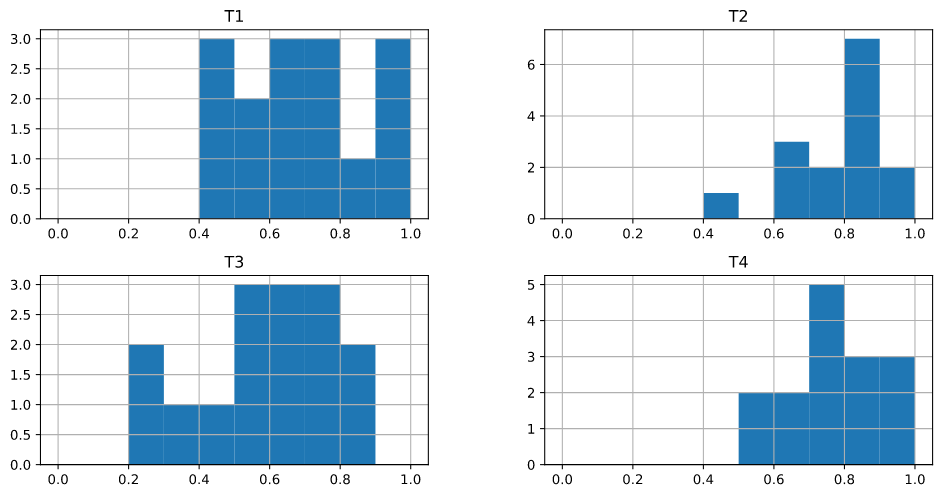
\includegraphics[scale=0.25]{tourist_histogram.png}
    \caption{Distributions of initial preferences of $T_1$, $T_2$, $T_3$ and $T_4$}
    \label{fig:tourist_hist} 
\end{figure}

For our experiments, the same relevances are shared between synthetic users, however future work should evaluate different relevances for each user tested. These relevances are shown on Table \ref{table:relevances-experiment}.

\begin{table*}[h!]
\centering
\caption{Simulated relevance of context factors for $T_1, T_2, T_3, T_4$
%Centroids to be used as simulated users.
}
\label{table:relevances-experiment}
\begin{tabular}{ |c|c|c|c|c|c|c|c|c|c| } 
    \hline
    \textbf{Class} & \textbf{rainy} & \textbf{cloudless} & \textbf{snowy} & \textbf{workday} & \textbf{weekend} & \textbf{morning} & \textbf{afternoon} & \textbf{night} & \textbf{early morning} \\
    \hline
    \hline

    Museum & 1.0 & 1.394 & 1.029 & 1.082 & 1.488 & 1.065 & 1.518 & 0.788 & 0.194 \\ \hline
    
    Interpretation Centre & 0.871 & 1.312 & 0.829 & 1.029 & 1.424 & 1.029  & 1.382 & 0.771 & 0.135 \\ \hline

    Libreary & 1.271 & 1.388  & 1.188  & 1.312 &1.159 & 1.324 & 1.453 & 0.729  & 0.271 \\ \hline

    Park and garden &
    0.335 & 1.847  & 0.894 & 1.365 & 1.665 & 1.388  & 1.629 & 0.924 & 0.494  \\ \hline

    Archeological Site &
    0.476 & 1.488 & 0.671 & 0.782 & 1.471 & 1.235 & 1.424 & 0.682  & 0.335 \\ \hline

    Religious Site &
    0.8 & 1.018 & 0.841  & 0.641  & 1.106 & 1.018 & 0.971 & 0.529  & 0.1 \\ \hline

    Remarkable building &
    0.912 & 1.576  & 0.994  & 1.165 & 1.506 & 1.241  & 1.453 & 1.0056 & 0.324 \\ \hline
    
    City heritage &
    0.665 & 1.629  & 0.947  & 1.088  & 1.618 & 1.329  & 1.565 & 1.271 & 0.5 \\ \hline
    
    Defense Site &
    0.712 & 1.412 & 0.806 & 0.835  & 1.376  & 1.253 & 1.388  & 0.824 & 0.265 \\ \hline
    
    Remembrance Site &
    0.588  & 1.318 & 0.812 & 0.935  & 1.306 & 1.129  & 1.294  & 0.6 & 0.324 \\ \hline
    
    Technical Heritage &
    0.582  & 1.371 & 0.682  & 0.841  & 1.3 & 1.265 & 1.3 & 0.741  & 0.3 \\ \hline
    
    Food Stablishment &
    1.488  & 1.624 & 1.494  & 1.635  & 1.759 & 1.353 & 1.671 & 1.676  & 0.688  \\ \hline
    
    Natural Heritage &
    0.494  & 1.776 & 0.835  & 1.088  & 1.659 & 1.535  & 1.524 & 0.953 & 0.465 \\ \hline
    
    Leisure place &
    1.088  & 1.541  & 1.006 & 1.118 & 1.588  & 1.024 & 1.506 & 1.418 & 0.588  \\ \hline
    
    Sports &
    0.1 & 2.0 & 0.75 & 1.118 & 1.588  & 1.024 & 1.506 & 0.8 & 0.588  \\ \hline
    
    Store &
    1.312 & 1.535  & 1.241  & 1.388  & 1.435  &1.0588  & 1.547  & 1.1647  & 0.3 \\ \hline


\end{tabular}
\end{table*}

For each tourist $T_i$, we simulate two visits to Niza, Lyon, and Paris for each possible combination of context factors values (Figure \ref{fig:experiments}), resulting in a total of $48$ visits by each $T_i$ to each place, which gives a total of $144$ visits by each $T_i$. The system returns a set of not more than $5$ recommended places inside a radius of $8$ kilometers for each visit; this set is going to be called the \textit{recommendation set}. 

\begin{figure}[h]
\centering
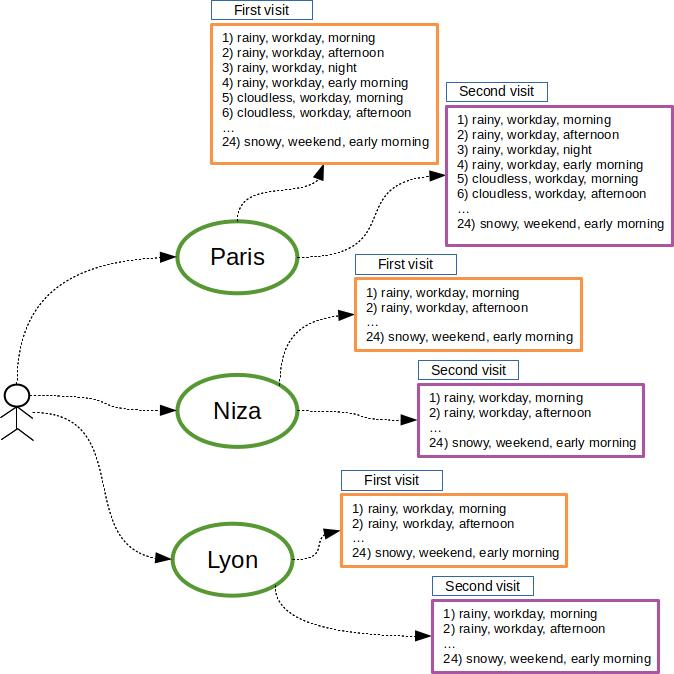
\includegraphics[scale=0.5]{draws/experiments.jpg}
\caption{Simulated visits}
\label{fig:experiments}
\end{figure}

\subsection{Metrics} \label{section:metrics}

Let $R$ be a recommendation set for a specific user on a specific location and a specific context (combination of context factors values), we define some metrics to evaluate how "good" is a \textit{recommendation} $R$, as follows:
%the following recommendation metrics:

\begin{itemize}
    \item Average preference of $R$ (Eq. (\ref{eq:pref_r})), which denotes how near to the user's preferences are the recommended POIs.
    \begin{equation} \label{eq:pref_r}
        pref_{R} = \frac{ \displaystyle \sum_{p \in R}{pref_p} }{| R |}
    \end{equation}

    \item Average activation of $R$ (Eq. (\ref{eq:act_r})), which denotes how relevant to the user are the current context factors values to the recommended POIs.
    \begin{equation} \label{eq:act_r}
        act_{R} = \frac{ \displaystyle \sum_{p \in R}{act_p} }{| R |}
    \end{equation}

    \item Average aging of $R$ (Eq. (\ref{eq:eta_r})), which denotes how "aged" to the user are the recommended POIs.
    \begin{equation} \label{eq:eta_r}
        \eta_{R} = \frac{ \displaystyle \sum_{p \in R}{\eta_p} }{| R |}
    \end{equation}

    \item Average distance of $R$ (Eq. (\ref{eq:dist_r})), which denotes how distant are the recommended POIs from the user.
    \begin{equation} \label{eq:dist_r}
        dist_{R} = \frac{ \displaystyle \sum_{p \in R}{dist_{p}} }{| R |}
    \end{equation}

    \item Average novelty of $R$ (Eq. (\ref{eq:nov_r})), which denotes how novel are the recommended POIs to the user. It uses Eq. (\ref{eq:novelty}), based on the work of Kotkov et al. \cite{kotkov2016survey}, where $p$ is a recommended place, $rec$ is the set of already recommended places to the user, $c_p$ is the ontology class to which $p$ belongs, and $dist$ computes the distance in the ontology (using \textit{Breadth First Search}) of two ontology classes.
    \begin{equation} \label{eq:novelty}
        nov_{p} = \  \underaccent{q \in rec}{min} \  ( dist( c_p, c_q ) )
    \end{equation}
    \begin{equation} \label{eq:nov_r}
        nov_{R} = \frac{ \displaystyle \sum_{p \in R}{nov_{p}} }{| R |}
    \end{equation}
\end{itemize}

\subsection{Experiments} \label{section:experiments}

To calculate the score for each POI $p$, we need some user-defined parameters, that represent maximum distance ($maxdist$) from the user to the PIO and the weighs ($w_i$) for each term in Eq. (\ref{eq:score})   (see Section \ref{section:score}). We designed two scenarios with different values of these configuration parameters, as we explain in the following.

\subsubsection{First configuration} 
\label{section:experiment-1}
We consider $maxdist =8 Km$, $w_1 = 0.3611$ for preference, $w_2 = 0.3611$ for activation, $w_3 = 0.25$ for aging, and $w_4 = 0.0278$ for distance from user, resulting on 
Eq. (\ref{eq:score-1}). In this configuration, we give
more priority to preference and activation and very little priority to distance from user. With these parameters we start simulating each user and their visits.

\begin{equation} \label{eq:score-1}
    \begin{split}
        score_p = \ &0.3611 \cdot pref_c + 0.3611 \cdot act_c \\
                                        &+ 0.25 \cdot \eta_p - 0.0278 \cdot \frac{dist_{u,p}}{8}
    \end{split}
\end{equation}


\textcolor{blue}{Hace falta una tablita que muestre los contextos y las preferencias de cada Ti , y quizás también el weather real y la configuración (por configuración).
Y en las tablas de recommendaciones poner pi (el sitio) y Quizás para que no hayan tantas tablas se puede hacer solo una con todas las visitas por turista y mostrar los 4 turistas. Podemos habla para decidir cómo irían las tablas.}

\textcolor{red}{Tenemos que buscar una manera de mostrar los resultados que sea más fácil de entender}

We are showing some sets of recommended items like Table \ref{table:t1-1}, where each $p_i$ is a recommended place and $score_{p_i} \ge score_{p_j}$ for every $i < j$. Table \ref{table:t1-1} corresponds to $T_1$'s first visit to Niza, on a rainy workday in the morning, where $p_1$ is Train des Merveilles (from class \textit{TouristTrain}), $p_2$ is Cinéma de Plein Air (from class \textit{Cinema}), $p_3$ is Casino de Beaulieu (from class \textit{Casino}), $p_4$ is Cinéma de Beaulieu (from class \textit{Cinema}) and $p_5$ is Lyon-style petanque fields (from class \textit{BoulesPitch}). We can see that since each of the places' ontology classes are subclasses of \textit{LeisurePlace}, which $T_1$ loves, they have same preference and activation and since this is the first recommendation, all aging values are $1.0$. Therefore, the distance is the tiebreaker. Despite of a rainy morning, the system recommends a tourist train to $T_1$, just because it is a leisure place.
\begin{table}[h!]
    \centering
    \begin{tabular}{ |c|c|c|c|c|c| } 
        \hline
        Field   & $p_1$ & $p_2$ & $p_3$ & $p_4$ & $p_5$ \\
        \hline
        $pref_c$    &  0.9353 & 0.9353 & 0.9353 & 0.9353 & 0.9353 \\
        $act_c$     & 4.4 & 4.4 & 4.4 & 4.4 & 4.4 \\
        $\eta_p$    & 1.0 & 1.0 & 1.0 & 1.0 & 1.0 \\
        $dist_{u,p}$ & 1.53 & 3.99 & 5.52 & 5.53 & 5.58 \\
        $score_p$    & 2.1713 & 2.1628 & 2.15745 & 2.15742 & 2.1573 \\
        
        \hline
    \end{tabular}
    \caption{First visit of $T_1$ to Niza with first configuration}
    \label{table:t1-1}
\end{table}


At the second visit to Lyon (see table \ref{table:t1-3}), on a rainy workday in the morning, only $p_1$ is not a leisure place but an interpretation center, a kind of place $T_1$ does not like as much as leisure places. However, the activation of \textit{InterpretationCenter} is higher enough to make $score_{p_1}$ greater than $score_{p_2}$. Despite of $p_1$ being very far away from $T_1$'s location, the little magnitude of $k_4$ makes it little important to the final score. Something odd on the recommended set is that $p_3$ and $p_4$ are the same place, Le Sucre, but reported as belonging to two different ontology classes: \textit{NightClub} and \textit{Theatre}, respectively.

\begin{table}[h!]
    \centering
    \begin{tabular}{ |c|c|c|c|c|c| } 
        \hline
        Field   & $p_1$ & $p_2$ & $p_3$ & $p_4$ & $p_5$ \\
        \hline
        $pref_c$    & 0.676 & 0.9353 & 0.9353 & 0.9353 & 0.9353 \\
        $act_c$     & 4.818 & 4.51 & 4.51 & 4.51 & 4.51 \\
        $\eta_p$    & 1.0 & 1.0 & 1.0 & 1.0 & 1.0 \\
        $dist_{u,p}$ & 7.1 & 4.45 & 4.54 & 4.54 & 4.61 \\
        $score_p$    & 2.2092 & 2.2015 & 2.2012 & 2.2012 & 2.2010 \\
        
        \hline
    \end{tabular}
    \caption{Second visit of $T_1$ to Lyon with first configuration}
    \label{table:t1-3}
\end{table}

At the fourth visit to Niza, on a rainy workday in the early morning, the system recommends table \ref{table:t1-2} to $T_1$, where $p_1$ is Cinéma de Plein Air (from class \textit{Cinema}), $p_2$ is Ferronnerie d'art JC Rodriguez (from class \textit{CraftsmanShop}), $p_3$ is Atelier Hesperida (from class \textit{CraftsmanShop}), $p_4$ is Horlogerie Foltête	(from class \textit{CraftsmanShop}) and $p_5$ is Galerie Bizet (from class \textit{CraftsmanShop}). Since $T_1$ loves leisure places more than stores, the predicted preference for Cinéma de Plein Air is greater than the other ones on this visit. However, we can see that $\eta_{p_1}$ lowers down $score_{p_1}$ to a value not so different from $score_{p_2}$. Cinéma de Plein Air does not appear again before a snowy workday afternoon, due to its aging and the $T_1$'s context.

\begin{table}[h!]
    \centering
    \begin{tabular}{ |c|c|c|c|c|c| } 
        \hline
        Field   & $p_1$ & $p_2$ & $p_3$ & $p_4$ & $p_5$ \\
        \hline
        $pref_c$    &  0.9353 & 0.7647 & 0.7647 & 0.7647 & 0.7647 \\
        $act_c$     & 4.2 & 4.1 & 4.1 & 4.1 & 4.1 \\
        $\eta_p$    & 0.6 & 1.0 & 1.0 & 1.0 & 1.0 \\
        $dist_{u,p}$ & 3.99 & 5.21 & 5.25 & 5.72 & 5.737 \\
        $score_p$    & 1.9906 & 1.9886 & 1.9884 & 1.98684 & 1.98678 \\
        
        \hline
    \end{tabular}
    \caption{Fourth visit of $T_1$ to Niza with first configuration}
    \label{table:t1-2}
\end{table}

While the system recommends same places to $T_1$ and $T_2$ for their first visits to Niza, Lyon and Paris, at rainy workdays at afternoon, the sets start to diverge after the second visits. The system recommends to $T_1$ a set of leisure places and one interpretation center for the second visit to Lyon, but recommends a set with two archeological sites, one interpretation center and two remarkable buildings to $T_2$, in that order (see table \ref{table:t2-1}). The more diverse initial preferences of $T_2$ and the aging system are responsible for this.

\begin{table}[h!]
    \centering
    \begin{tabular}{ |c|c|c|c|c|c| } 
        \hline
        Field   & $p_1$ & $p_2$ & $p_3$ & $p_4$ & $p_5$ \\
        \hline
        $pref_c$    &  0.852 & 0.852 & 0.659 & 0.843 & 0.843 \\
        $act_c$     & 4.659 & 4.659 & 4.818 & 4.6 & 4.6 \\
        $\eta_p$    & 1.0 & 1.0 & 1.0 & 1.0 & 1.0 \\
        $dist_{u,p}$ & 3.967 & 5.267 & 7.0969 & 3.967 & 5.267 \\
        $score_p$    & 2.226 & 2.222 & 2.203 & 2.202 & 2.197 \\
        
        \hline
    \end{tabular}
    \caption{Second visit of $T_2$ to Lyon with first configuration}
    \label{table:t2-1}
\end{table}

After many visits, again at a rainy workday at afternoon, the system recommends a completely different set of places to $T_2$ when visiting Lyon again. It recommends a theater, an art gallery, a craftsman shop and two other art galleries, in that order (see table \ref{table:t2-2}). The system aging is responsible for this variety of recommendations.
\begin{table}[h!]
    \centering
    \begin{tabular}{ |c|c|c|c|c|c| } 
        \hline
        Field   & $p_1$ & $p_2$ & $p_3$ & $p_4$ & $p_5$ \\
        \hline
        $pref_c$    &  0.843 & 0.829 & 0.829 & 0.829 & 0.829 \\
        $act_c$     & 4.512 & 4.371 & 4.371 & 4.371 & 4.371 \\
        $\eta_p$    & 0.8 & 1.0 & 1.0 & 1.0 & 1.0 \\
        $dist_{u,p}$ & 7.157 & 5.425 & 5.438 & 5.442 & 5.462 \\
        $score_p$    & 2.10876 & 2.10864 & 2.10859 & 2.10858 & 2.10851 \\
        
        \hline
    \end{tabular}
    \caption{A visit of $T_2$ to Lyon with first configuration after many visits}
    \label{table:t2-2}
\end{table}

However, there are cases where $k_3$ is not high enough to make more diverse the recommendations, as in the two visits of $T_2$ to Paris on cloudless workdays at early morning (see tables \ref{table:t2-3} and \ref{table:t2-4}), where the second one is made after many visits. Both visits involve Garnier Opera (from class \textit{Palace}), Conciergerie (from class \textit{Palace}) and Le Manoir de Paris (from class \textit{InterpretationCentre}), as $p_2$, $p_3$ and $p_4$ for the first visit and $p_1$, $p_5$ and $p_2$ for the second visit, respectively.

\begin{table}[h!]
    \centering
    \begin{tabular}{ |c|c|c|c|c|c| } 
        \hline
        Field   & $p_1$ & $p_2$ & $p_3$ & $p_4$ & $p_5$ \\
        \hline
        $pref_c$    &  0.829 & 0.843 & 0.843 & 0.659 & 0.659 \\
        $act_c$     & 4.171 & 4.4 & 4.4 & 4.571 & 4.571 \\
        $\eta_p$    & 0.8 & 0.4 & 0.4 & 0.4 & 0.4 \\
        $dist_{u,p}$ & 7.51 & 4.25 & 5.06 & 5.9 & 6.3 \\
        $score_p$    & 1.97916 & 1.97869 & 1.97590 & 1.96803 & 1.96665 \\
        
        \hline
    \end{tabular}
    \caption{First visit of $T_2$ to Paris with first configuration on a cloudless workday at early morning}
    \label{table:t2-3}
\end{table}

\begin{table}[h!]
    \centering
    \begin{tabular}{ |c|c|c|c|c|c| } 
        \hline
        Field   & $p_1$ & $p_2$ & $p_3$ & $p_4$ & $p_5$ \\
        \hline
        $pref_c$    &  0.843 & 0.843 & 0.659 & 0.659 & 0.659 \\
        $act_c$     & 4.40 & 4.40 & 4.57 & 4.57 & 4.57  \\
        $\eta_p$    & 0.4 & 0.4 & 0.4 & 0.4 & 0.4 \\
        $dist_{u,p}$ & 4.25 & 5.06 & 3.79 & 4.55 & 5.9 \\
        $score_p$    & 1.97869 & 1.97590 & 1.97535 & 1.97273 & 1.96803 \\
        
        \hline
    \end{tabular}
    \caption{Second visit of $T_2$ to Paris with first configuration on a cloudless workday at early morning}
    \label{table:t2-4}
\end{table}

Table \ref{table:config-1} shows the average of the recommendation metrics for each tourist using first configuration. Averages of $pref_R$ of $T_1$'s and $T_2$'s visits are the highest ones, being greater than $0.8$ and hence closer to $1.0$, the maximum possible value. Next is $T_4$'s, being greater than $0.7$, which is still a good average preference. $T_3$'s average $pref_R$ is lower, but we can blame the amount of low initial preferences of $T_3$, as we can see on figure \ref{fig:tourist_hist}.
\begin{table}[h!]
    \centering
    \begin{tabular}{ |c|c|c|c|c| } 
        \hline
        avg & $T_1$ & $T_2$ & $T_3$ & $T_4$ \\
        \hline
        \hline
        $avg(pref_R)$ & 0.8555 & 0.8213 & 0.4183 & 0.7269\\
        $avg(act_R)$ & 4.286 & 4.3092 & 4.314 & 4.3319 \\
        $avg(\eta_R)$ & 0.7058 & 0.7111 & 0.6906 & 0.6914 \\
        $avg(nov_{u,R})$ & 0.0923 & 0.1231 & 0.1329 & 0.1147 \\
        $avg(dist_{u,R})$ & 4.876 & 4.8993 & 4.9101 & 4.9861 \\
       
        \hline
    \end{tabular}
    \caption{Averages of recommendations metrics with first configuration}
    \label{table:config-1}
\end{table}

The average $act_R$ of each tourist is greater than $4.0$. Theoretically, the maximum possible value is $6.0$, but since the relevance values obtained by the survey (see section \ref{section:relevances-survey}) do not reach their maximum possible value, which is $2.0$, it is impossible for these experiments.

Average $\eta_R$ is very near $0.7$, hence the amount of "young" recommended places is high. Theoretically, the maximum possible value is $1.0$, but that would be possible if each recommendation involves POIs never recommended before. 

Despite of recommending places with distance from user near $8.0$ km, the average $dist_{u,R}$ for each tourist is acceptable: greater than $4.0$ km and less than $5.0$ km. The novelties measured as we proposed on section \ref{section:metrics} have bad performance on four tourists.

\subsubsection{Second configuration} \label{section:experiment-2}
Now we consider $k_1 = \frac{1}{4}$ for preference, $k_2 = \frac{1}{4}$ for activation, $k_3 = \frac{1}{4} + \frac{2}{9}$ for aging and $k_4 = \frac{1}{4} - \frac{2}{9}$ for distance from user, resulting on equation \ref{eq:score-2} and giving now more priority to aging.
\begin{equation} \label{eq:score-2}
    \begin{split}
        score_p = \ &\frac{1}{4} \cdot pref_c + \frac{1}{4} \cdot act_c \\
                                        &+ \frac{17}{36} \cdot \eta_p - \frac{1}{36} \cdot \frac{dist_{u,p}}{8}
    \end{split}
\end{equation}

For the first visit of $T_1$ to Niza in a cloudless workday at afternoon, the $\eta_R$ is $0.84$ using the second configuration (see table \ref{table:2nd-t1-niza-1}), while it is $0.80$ using the first configuration (see table \ref{table:1st-t1-niza-1}). Even the $pref_R$ improve, from $0.765$ to $0.799$, but the $act_R$ goes from $4.44$ to $4.33$.

\begin{table}[h!]
    \centering
    \begin{tabular}{ |c|c|c|c|c|c| } 
        \hline
        Field   & $p_1$ & $p_2$ & $p_3$ & $p_4$ & $p_5$ \\
        \hline
        $pref_c$    &  0.76 & 0.76 & 0.76 & 0.76 & 0.76 \\
        $act_c$     & 4.44 & 4.44 & 4.44 & 4.44 & 4.44  \\
        $\eta_p$    & 0.8 & 0.8 & 0.8 & 0.8 & 0.8 \\
        $dist_{u,p}$ & 5.25 & 5.72 & 5.74 & 5.78 & 5.79 \\
        $score_p$    & 2.06166 & 2.06004 & 2.05998 & 2.05983 & 2.05981 \\
        
        \hline
    \end{tabular}
    \caption{First visit of $T_1$ to Niza with first configuration on a cloudless workday at afternoon}
    \label{table:1st-t1-niza-1}
\end{table}

\begin{table}[h!]
    \centering
    \begin{tabular}{ |c|c|c|c|c|c| } 
        \hline
        Field   & $p_1$ & $p_2$ & $p_3$ & $p_4$ & $p_5$ \\
        \hline
        $pref_c$    &  0.76 & 0.76 & 0.935 & 0.76 & 0.76 \\
        $act_c$     & 4.44 & 4.44 & 3.89 & 4.44 & 4.44  \\
        $\eta_p$    & 0.8 & 0.8 & 1.0 & 0.8 & 0.8 \\
        $dist_{u,p}$ & 5.20 & 5.25 & 5.30 & 5.72 & 5.73 \\
        $score_p$    & 1.6612 & 1.6610 & 1.6597 & 1.6594 & 1.6593 \\
        
        \hline
    \end{tabular}
    \caption{First visit of $T_1$ to Niza with second configuration on a cloudless workday at afternoon}
    \label{table:2nd-t1-niza-1}
\end{table}

For the second visit of $T_4$ to Paris on a snowy weekend at early morning, the $\eta_R$ is $0.774$ using second configuration (see table \ref{table:1st-t4-Paris-2}), while it is $0.691$ using first configuration (see table \ref{table:2nd-t4-Paris-2}). The $pref_R$ and the $act_R$ decrease from $0.727$ to $0.699$ and from $4.332$ to $4.041$, respectively.

\begin{table}[h!]
    \centering
    \begin{tabular}{ |c|c|c|c|c|c| } 
        \hline
        Field   & $p_1$ & $p_2$ & $p_3$ & $p_4$ & $p_5$ \\
        \hline
        $pref_c$    &  0.866 & 0.866 & 0.790 & 0.866 & 0.866 \\
        $act_c$     & 4.288 & 4.288 & 4.265 & 4.288 & 4.288  \\
        $\eta_p$    & 0.4 & 0.4 & 0.4 & 0.2 & 0.2 \\
        $dist_{u,p}$ & 5.899 & 6.297 & 4.253 & 3.791 & 4.546 \\
        $score_p$    & 1.941 & 1.939 & 1.911 & 1.898 & 1.895 \\
        
        \hline
    \end{tabular}
    \caption{Second visit of $T_4$ to Paris with first configuration on a snowy weekend at early morning}
    \label{table:1st-t4-Paris-2}
\end{table}

\begin{table}[h!]
    \centering
    \begin{tabular}{ |c|c|c|c|c|c| } 
        \hline
        Field   & $p_1$ & $p_2$ & $p_3$ & $p_4$ & $p_5$ \\
        \hline
        $pref_c$    &  0.866 & 0.866 & 0.738 & 0.866 & 0.866 \\
        $act_c$     & 4.288 & 4.288 & 3.81 & 4.288 & 4.288  \\
        $\eta_p$    & 1.0 & 1.0 & 0.6 & 0.2 & 0.2 \\
        $dist_{u,p}$ & 3.791 & 4.546 & 5.333 & 5.899 & 6.297 \\
        $score_p$    & 1.748 & 1.745 & 1.402 & 1.363 & 1.361 \\
        
        \hline
    \end{tabular}
    \caption{Second visit of $T_4$ to Paris with second configuration on a snowy weekend at early morning}
    \label{table:2nd-t4-Paris-2}
\end{table}

Table \ref{table:config-2} shows the average of the recommendation metrics for each tourist using second configuration. Again, $T_1$'s and $T_2$'s $avg(pref_R)$ are the highest ones, followed by $T_4$'s, while $T_3$'s is the lowest. We can notice that only $T_1$'s and $T_2$'s $avg(pref_R)$ increase a little from the ones with first configuration, but the other two decrease. Again, all $avg(act_R)$ are above $4.0$, but each one decreases from the first configuration version. As expected, all $avg(\eta_R)$ increase because the second configuration gives more weight to aging.

\begin{table}[h!]
    \centering
    \begin{tabular}{ |c|c|c|c|c| } 
        \hline
        avg & $T_1$ & $T_2$ & $T_3$ & $T_4$ \\
        \hline
        \hline
        $avg(pref_R)$ & 0.8658 & 0.8272 & 0.3912 & 0.6987 \\
        $avg(act_R)$ & 4.0738 & 4.0818 & 4.0031 & 4.0415 \\
        $avg(\eta_R)$ & 0.7592 & 0.7619 & 0.7850 & 0.7739 \\
        $avg(nov_{u,R})$ & 0.172 & 0.1860 & 0.1986 & 0.1580 \\
        $avg(dist_{u,R})$ & 4.842 & 5.0215 & 4.8999 & 4.9615 \\
       
        \hline
    \end{tabular}
    \caption{Averages of recommendations metrics with second configuration}
    \label{table:config-2}
\end{table}

\subsubsection{Discussion}

For measuring novelty we use the Eq. (\ref{eq:novelty}) based on Kotkov et al. \cite{kotkov2016survey}, since when novelty increases, so does serendipity. That equation was proposed with the hypotheses that if a user already knows places from class $c$, then it is probable the user already knows other places from class $c$. With that hypotheses, our system gives poor novelty: when a place belonging to the ontology class $c$ is recommended, next recommendations with places from $c$ will have lower novelty. However, considering average aging as a good metric for the level of variability, both experiments on section \ref{section:experiments} give high average aging, which means a lot of "young" or not frequently recommended places are returned to the user, which could imply an increment on system serendipity. Future work should try more advanced ways for measuring serendipity.

Of course, experiment \ref{section:experiment-2} is focused on increasing average aging by giving a higher value to $k_3$ on Eq. (\ref{eq:score}), but the increment of aging is paid with a decrement on activation. Nonetheless, two simulated tourists have an increment for their preferences, because on first configuration the system is trapped between very activated POIs but not very relevant, but the heavier aging of the second configuration increases variability, hence lets the system recommend other POIs despite of lowering the activation. 

Nevertheless, a deployed version of this system should let the users choose each $w_i$ of Eq. (\ref{eq:score}), that way choosing if they want recommendations mainly relevant than contextually activated or varied, or even recommendations with the nearest places ignoring any other attribute, or any other possible configuration.